\documentclass{article}

\usepackage{amsmath}
\usepackage{amssymb}
\usepackage{amsthm}

\usepackage{tikz}
\usepgflibrary{shapes.arrows}
\usepgflibrary{shapes.geometric}
\usepgflibrary{shapes.symbols}

\setlength{\pdfpagewidth}{15.1cm}
\setlength{\pdfpageheight}{12.6cm}
%\setlength{\pdfvorigin}{25.4mm}

%\setlength{\textwidth}{16cm}
%\setlength{\textheight}{23cm}
\setlength{\evensidemargin}{0cm}
\setlength{\oddsidemargin}{-3.1cm}
\setlength{\topmargin}{-2.45cm}
\setlength{\headheight}{0cm}
\setlength{\headsep}{0cm}

\pagestyle{empty}

\newcommand{\derivnuc}[2]{\frac{\partial}{\partial #1_#2}}

\begin{document}

\begin{tikzpicture}[style=very thick]
  % root
  \node (root) at (6,4.5) [draw,shape=circle,color=red,fill=red!10,inner sep=1pt] {\textbf{1(1)}};
  % the 2nd level
  \node (level20) at (3,3) [draw,shape=circle,color=red,fill=red!10,inner sep=1pt] {\textbf{1(1)}};
  \draw [->,color=red] (root) -- (level20) node [midway,above,color=red] {\textbf{0}};
  \node (level21) at (6,3) [draw,shape=circle,inner sep=1pt] {\textbf{2(2)}};
  \draw [->] (root) -- (level21) node [midway,left] {\textbf{1}};
  \node (level22) at (7,3) [draw,shape=circle,inner sep=1pt] {\textbf{3(2)}};
  \draw [->] (root) -- (level22) node [midway,right] {\textbf{1}};
  % the 3rd level
  \node (level30) at (1,1.5) [draw,shape=circle,inner sep=1pt] {\textbf{1(1)}};
  \draw [->] (level20) -- (level30) node [midway,above] {\textbf{0}};
  \node (level31) at (3,1.5) [draw,shape=circle,color=red,fill=red!10,inner sep=1pt] {\textbf{2(2)}};
  \draw [->,color=red] (level20) -- (level31) node [midway,left,color=red] {\textbf{1}};
  \node (level32) at (4,1.5) [draw,shape=circle,inner sep=1pt] {\textbf{3(2)}};
  \draw [->] (level20) -- (level32) node [midway,right] {\textbf{1}};
  \node (level33) at (6,1.5) [draw,shape=circle,inner sep=1pt] {\textbf{2(2)}};
  \draw [->] (level21) -- (level33) node [midway,left] {\textbf{0}};
  \node (level34) at (7,1.5) [draw,shape=circle,inner sep=1pt] {\textbf{3(3)}};
  \draw [->] (level21) -- (level34) node [midway,right] {\textbf{1}};
  \node (level35) at (8,1.5) [draw,shape=circle,inner sep=1pt] {\textbf{3(2)}};
  \draw [->] (level22) -- (level35) node [midway,right] {\textbf{0}};
 % the 4th level
  \node (leaf0) at (0,0) [draw,shape=circle,inner sep=1pt] {\textbf{1(1)}};
  \draw [->] (level30) -- (leaf0) node [midway,left] {\textbf{0}};
  \node (leaf1) at (1,0) [draw,shape=circle,inner sep=1pt] {\textbf{2(2)}};
  \draw [->] (level30) -- (leaf1) node [midway,left] {\textbf{1}};
  \node (leaf2) at (2,0) [draw,shape=circle,inner sep=1pt] {\textbf{3(2)}};
  \draw [->] (level30) -- (leaf2) node [midway,right] {\textbf{1}};
  \node (leaf3) at (3,0) [draw,shape=circle,color=red,fill=red!10,inner sep=1pt] {\textbf{2(2)}};
  \draw [->,color=red] (level31) -- (leaf3) node [midway,left,color=red] {\textbf{0}};
  \node (leaf4) at (4,0) [draw,shape=circle,inner sep=1pt] {\textbf{3(3)}};
  \draw [->] (level31) -- (leaf4) node [midway,right] {\textbf{1}};
  \node (leaf5) at (5,0) [draw,shape=circle,inner sep=1pt] {\textbf{3(2)}};
  \draw [->] (level32) -- (leaf5) node [midway,right] {\textbf{0}};
  \node (leaf6) at (6,0) [draw,shape=circle,inner sep=1pt] {\textbf{2(2)}};
  \draw [->] (level33) -- (leaf6) node [midway,left] {\textbf{0}};
  \node (leaf7) at (7,0) [draw,shape=circle,inner sep=1pt] {\textbf{3(3)}};
  \draw [->] (level33) -- (leaf7) node [midway,right] {\textbf{1}};
  \node (leaf8) at (8,0) [draw,shape=circle,inner sep=1pt] {\textbf{3(3)}};
  \draw [->] (level34) -- (leaf8) node [midway,right] {\textbf{0}};
  \node (leaf9) at (9,0) [draw,shape=circle,inner sep=1pt] {\textbf{3(2)}};
  \draw [->] (level35) -- (leaf9) node [midway,right] {\textbf{0}};
  % height of the tree
  \draw [-] (root) -- (10,4.5);
  \draw [-] (leaf9) -- (10,0);
  \node (height) at (9.75,2.5) {$H=3$};
  \node (order) at (9.75,2) {$L\equiv H+1=4$};
  \draw [->] (height) -- (9.75,4.5);
  \draw [->] (order) -- (9.75,0);
  % chosen centers
  \node (centers) at (3,-2.06) [draw,shape=rectangle,inner sep=5pt,color=red,fill=red!10]%
    {$\underbrace{\mathbf{1\qquad1}}_{|\boldsymbol{L}_{1}|=2}\qquad\underbrace{\mathbf{2\qquad2}}_{|\boldsymbol{L}_{2}|=2}$};
  \node at (3,-0.9) [single arrow,fill=red!80,rotate=270,single arrow head indent=0.5ex,minimum height=1cm] {};
  % triangular derivatives of the 1st center
  \node at (-1.6,-4) {$\displaystyle\binom{|\boldsymbol{L}_{1}|+2}{2}$};
  \node at (1.5,-3.2) [single arrow,fill=red!80,rotate=220,single arrow head indent=0.5ex,minimum height=1.5cm] {};
  \node [regular polygon, regular polygon sides=3, minimum size=6.2cm, draw, color=red, nearly transparent, fill=red] at (0.2,-5.8) {};
  \node [color=red] (xx2) at (0.2,-4.2) {$\displaystyle\derivnuc{X}{1}\derivnuc{X}{1}$};
  \node [color=red] (xy2) at (-0.6,-5.5) {$\displaystyle\derivnuc{X}{1}\derivnuc{Y}{1}$};
  \node [color=red] (xz2) at (1,-5.5) {$\displaystyle\derivnuc{X}{1}\derivnuc{Z}{1}$};
  \node [color=red] (yy2) at (-1.4,-6.8) {$\displaystyle\derivnuc{Y}{1}\derivnuc{Y}{1}$};
  \node [color=red] (yz2) at (0.2,-6.8) {$\displaystyle\derivnuc{Y}{1}\derivnuc{Z}{1}$};
  \node [color=red] (zz2) at (1.8,-6.8) {$\displaystyle\derivnuc{Z}{1}\derivnuc{Z}{1}$};
  \draw [-,color=red] (2.8,-5.2) -- (3.2,-5.6);
  \draw [-,color=red] (2.8,-5.6) -- (3.2,-5.2);
  % triangular derivatives of the 2nd center
  \node at (7.6,-4) {$\displaystyle\binom{|\boldsymbol{L}_{2}|+2}{2}$};
  \node at (4.5,-3.2) [single arrow,fill=red!80,rotate=320,single arrow head indent=0.5ex,minimum height=1.5cm] {};
  \node [regular polygon, regular polygon sides=3, minimum size=6.2cm, draw, color=red, nearly transparent, fill=red] at (5.8,-5.8) {};
  \node [color=red] (xx1) at (5.8,-4.2) {$\displaystyle\derivnuc{X}{2}\derivnuc{X}{2}$};
  \node [color=red] (xy1) at (5,-5.5) {$\displaystyle\derivnuc{X}{2}\derivnuc{Y}{2}$};
  \node [color=red] (xz1) at (6.6,-5.5) {$\displaystyle\derivnuc{X}{2}\derivnuc{Z}{2}$};
  \node [color=red] (yy1) at (4.2,-6.8) {$\displaystyle\derivnuc{Y}{2}\derivnuc{Y}{2}$};
  \node [color=red] (yz1) at (5.8,-6.8) {$\displaystyle\derivnuc{Y}{2}\derivnuc{Z}{2}$};
  \node [color=red] (zz1) at (7.4,-6.8) {$\displaystyle\derivnuc{Z}{2}\derivnuc{Z}{2}$};
  % all the derivatives
  \node at (8.3,-5.5) [single arrow,fill=red!80,single arrow head indent=0.5ex,minimum height=1.5cm] {};
  \node at (10.8,-2.7) {$\displaystyle\prod_{k=1}^{\gamma=2}\binom{|\boldsymbol{L}_{k}|+2}{2}$};
  \node at (10.8,-5.4) [tape, draw, color=red, fill=red!20, text width=3cm, inner sep=4pt] %
    {$\displaystyle\derivnuc{X}{1}\derivnuc{X}{1}\derivnuc{X}{2}\derivnuc{X}{2}$
     $\qquad\text{ }\qquad\text{ }\qquad\text{ }\qquad\text{ }\qquad\text{ }\qquad\text{ }$
     $\displaystyle\derivnuc{X}{1}\derivnuc{Y}{1}\derivnuc{X}{2}\derivnuc{X}{2}$
     $\qquad\text{ }\qquad\text{ }\qquad\text{ }\qquad\text{ }\qquad\text{ }\qquad\text{ }$
     $\cdots\cdots\cdots\cdots\cdots\cdots$
     $\qquad\text{ }\qquad\text{ }\qquad\text{ }\qquad\text{ }\qquad\text{ }\qquad\text{ }$
     $\displaystyle\derivnuc{Z}{1}\derivnuc{Z}{1}\derivnuc{Z}{2}\derivnuc{Z}{2}$};
\end{tikzpicture}

\end{document}
